% Created by tikzDevice version 0.12.3.2 on 2022-02-15 15:49:54
% !TEX encoding = UTF-8 Unicode
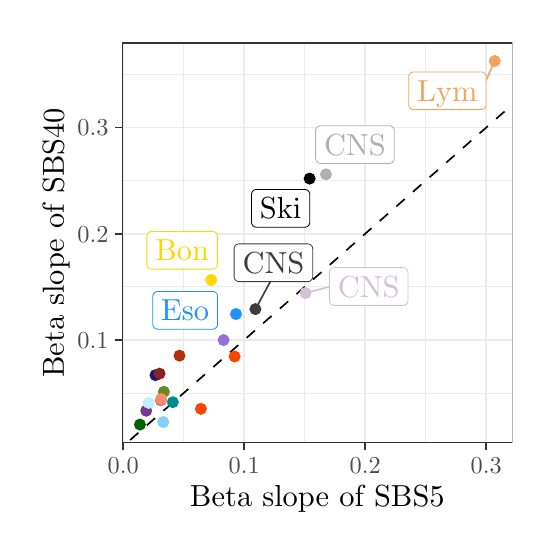
\begin{tikzpicture}[x=1pt,y=1pt]
\definecolor{fillColor}{RGB}{255,255,255}
\path[use as bounding box,fill=fillColor,fill opacity=0.00] (0,0) rectangle (180.67,180.67);
\begin{scope}
\path[clip] (  0.00,  0.00) rectangle (180.67,180.67);
\definecolor{drawColor}{RGB}{255,255,255}
\definecolor{fillColor}{RGB}{255,255,255}

\path[draw=drawColor,line width= 0.6pt,line join=round,line cap=round,fill=fillColor] (  0.00,  0.00) rectangle (180.68,180.68);
\end{scope}
\begin{scope}
\path[clip] ( 34.16, 30.69) rectangle (175.17,175.17);
\definecolor{fillColor}{RGB}{255,255,255}

\path[fill=fillColor] ( 34.16, 30.69) rectangle (175.17,175.17);
\definecolor{drawColor}{gray}{0.92}

\path[draw=drawColor,line width= 0.3pt,line join=round] ( 34.16, 48.66) --
	(175.17, 48.66);

\path[draw=drawColor,line width= 0.3pt,line join=round] ( 34.16, 87.04) --
	(175.17, 87.04);

\path[draw=drawColor,line width= 0.3pt,line join=round] ( 34.16,125.41) --
	(175.17,125.41);

\path[draw=drawColor,line width= 0.3pt,line join=round] ( 34.16,163.79) --
	(175.17,163.79);

\path[draw=drawColor,line width= 0.3pt,line join=round] ( 56.39, 30.69) --
	( 56.39,175.17);

\path[draw=drawColor,line width= 0.3pt,line join=round] (100.12, 30.69) --
	(100.12,175.17);

\path[draw=drawColor,line width= 0.3pt,line join=round] (143.86, 30.69) --
	(143.86,175.17);

\path[draw=drawColor,line width= 0.6pt,line join=round] ( 34.16, 67.85) --
	(175.17, 67.85);

\path[draw=drawColor,line width= 0.6pt,line join=round] ( 34.16,106.23) --
	(175.17,106.23);

\path[draw=drawColor,line width= 0.6pt,line join=round] ( 34.16,144.60) --
	(175.17,144.60);

\path[draw=drawColor,line width= 0.6pt,line join=round] ( 34.52, 30.69) --
	( 34.52,175.17);

\path[draw=drawColor,line width= 0.6pt,line join=round] ( 78.26, 30.69) --
	( 78.26,175.17);

\path[draw=drawColor,line width= 0.6pt,line join=round] (121.99, 30.69) --
	(121.99,175.17);

\path[draw=drawColor,line width= 0.6pt,line join=round] (165.72, 30.69) --
	(165.72,175.17);
\definecolor{drawColor}{RGB}{0,0,0}

\path[draw=drawColor,line width= 0.6pt,dash pattern=on 4pt off 4pt ,line join=round] (  0.93,  0.00) -- (180.67,157.72);
\definecolor{drawColor}{RGB}{255,215,0}
\definecolor{fillColor}{RGB}{255,215,0}

\path[draw=drawColor,line width= 0.4pt,line join=round,line cap=round,fill=fillColor] ( 66.30, 89.48) circle (  1.96);
\definecolor{drawColor}{RGB}{205,96,144}
\definecolor{fillColor}{RGB}{205,96,144}

\path[draw=drawColor,line width= 0.4pt,line join=round,line cap=round,fill=fillColor] ( 48.12, 46.02) circle (  1.96);
\definecolor{drawColor}{gray}{0.24}
\definecolor{fillColor}{gray}{0.24}

\path[draw=drawColor,line width= 0.4pt,line join=round,line cap=round,fill=fillColor] ( 82.29, 78.97) circle (  1.96);
\definecolor{drawColor}{RGB}{216,191,216}
\definecolor{fillColor}{RGB}{216,191,216}

\path[draw=drawColor,line width= 0.4pt,line join=round,line cap=round,fill=fillColor] (100.39, 84.79) circle (  1.96);
\definecolor{drawColor}{gray}{0.69}
\definecolor{fillColor}{gray}{0.69}

\path[draw=drawColor,line width= 0.4pt,line join=round,line cap=round,fill=fillColor] (107.78,127.67) circle (  1.96);
\definecolor{drawColor}{RGB}{25,25,112}
\definecolor{fillColor}{RGB}{25,25,112}

\path[draw=drawColor,line width= 0.4pt,line join=round,line cap=round,fill=fillColor] ( 46.18, 55.12) circle (  1.96);
\definecolor{drawColor}{RGB}{30,144,255}
\definecolor{fillColor}{RGB}{30,144,255}

\path[draw=drawColor,line width= 0.4pt,line join=round,line cap=round,fill=fillColor] ( 75.28, 77.20) circle (  1.96);
\definecolor{drawColor}{RGB}{139,35,35}
\definecolor{fillColor}{RGB}{139,35,35}

\path[draw=drawColor,line width= 0.4pt,line join=round,line cap=round,fill=fillColor] ( 47.66, 55.66) circle (  1.96);
\definecolor{drawColor}{RGB}{179,47,11}
\definecolor{fillColor}{RGB}{179,47,11}

\path[draw=drawColor,line width= 0.4pt,line join=round,line cap=round,fill=fillColor] ( 54.86, 62.15) circle (  1.96);
\definecolor{drawColor}{RGB}{255,69,0}
\definecolor{fillColor}{RGB}{255,69,0}

\path[draw=drawColor,line width= 0.4pt,line join=round,line cap=round,fill=fillColor] ( 74.79, 61.85) circle (  1.96);

\path[draw=drawColor,line width= 0.4pt,line join=round,line cap=round,fill=fillColor] ( 62.60, 42.94) circle (  1.96);
\definecolor{drawColor}{RGB}{0,100,0}
\definecolor{fillColor}{RGB}{0,100,0}

\path[draw=drawColor,line width= 0.4pt,line join=round,line cap=round,fill=fillColor] ( 40.57, 37.25) circle (  1.96);
\definecolor{drawColor}{RGB}{105,139,34}
\definecolor{fillColor}{RGB}{105,139,34}

\path[draw=drawColor,line width= 0.4pt,line join=round,line cap=round,fill=fillColor] ( 49.22, 49.10) circle (  1.96);
\definecolor{drawColor}{RGB}{244,163,93}
\definecolor{fillColor}{RGB}{244,163,93}

\path[draw=drawColor,line width= 0.4pt,line join=round,line cap=round,fill=fillColor] (168.77,168.61) circle (  1.96);
\definecolor{drawColor}{RGB}{0,139,139}
\definecolor{fillColor}{RGB}{0,139,139}

\path[draw=drawColor,line width= 0.4pt,line join=round,line cap=round,fill=fillColor] ( 52.45, 45.33) circle (  1.96);
\definecolor{drawColor}{RGB}{122,55,139}
\definecolor{fillColor}{RGB}{122,55,139}

\path[draw=drawColor,line width= 0.4pt,line join=round,line cap=round,fill=fillColor] ( 42.84, 42.24) circle (  1.96);
\definecolor{drawColor}{RGB}{135,206,250}
\definecolor{fillColor}{RGB}{135,206,250}

\path[draw=drawColor,line width= 0.4pt,line join=round,line cap=round,fill=fillColor] ( 49.00, 38.17) circle (  1.96);
\definecolor{drawColor}{RGB}{0,0,0}
\definecolor{fillColor}{RGB}{0,0,0}

\path[draw=drawColor,line width= 0.4pt,line join=round,line cap=round,fill=fillColor] (101.89,126.12) circle (  1.96);
\definecolor{drawColor}{RGB}{191,239,255}
\definecolor{fillColor}{RGB}{191,239,255}

\path[draw=drawColor,line width= 0.4pt,line join=round,line cap=round,fill=fillColor] ( 43.74, 45.08) circle (  1.96);
\definecolor{drawColor}{RGB}{147,112,219}
\definecolor{fillColor}{RGB}{147,112,219}

\path[draw=drawColor,line width= 0.4pt,line join=round,line cap=round,fill=fillColor] ( 70.80, 67.78) circle (  1.96);
\definecolor{drawColor}{RGB}{255,140,105}
\definecolor{fillColor}{RGB}{255,140,105}

\path[draw=drawColor,line width= 0.4pt,line join=round,line cap=round,fill=fillColor] ( 48.21, 46.46) circle (  1.96);
\end{scope}
\begin{scope}
\path[clip] ( 34.16, 30.69) rectangle (175.17,175.17);
\definecolor{drawColor}{gray}{0.24}

\path[draw=drawColor,line width= 0.6pt,line join=round,line cap=round] ( 87.69, 88.91) -- ( 82.73, 79.78);
\definecolor{drawColor}{RGB}{216,191,216}

\path[draw=drawColor,line width= 0.6pt,line join=round,line cap=round] (109.02, 87.05) -- (101.27, 85.02);
\definecolor{drawColor}{RGB}{244,163,93}

\path[draw=drawColor,line width= 0.6pt,line join=round,line cap=round] (165.63,161.60) -- (168.39,167.76);
\definecolor{drawColor}{RGB}{255,215,0}
\definecolor{fillColor}{RGB}{255,255,255}

\path[draw=drawColor,line width= 0.3pt,line join=round,line cap=round,fill=fillColor] ( 44.87, 93.41) --
	( 66.75, 93.41) --
	( 66.68, 93.41) --
	( 66.97, 93.43) --
	( 67.25, 93.48) --
	( 67.53, 93.59) --
	( 67.78, 93.73) --
	( 68.00, 93.92) --
	( 68.20, 94.13) --
	( 68.35, 94.38) --
	( 68.47, 94.65) --
	( 68.54, 94.93) --
	( 68.56, 95.22) --
	( 68.56, 95.22) --
	( 68.56,105.23) --
	( 68.56,105.23) --
	( 68.54,105.52) --
	( 68.47,105.80) --
	( 68.35,106.07) --
	( 68.20,106.32) --
	( 68.00,106.54) --
	( 67.78,106.72) --
	( 67.53,106.86) --
	( 67.25,106.97) --
	( 66.97,107.03) --
	( 66.75,107.04) --
	( 44.87,107.04) --
	( 45.09,107.03) --
	( 44.80,107.04) --
	( 44.51,107.00) --
	( 44.23,106.92) --
	( 43.97,106.80) --
	( 43.73,106.63) --
	( 43.52,106.43) --
	( 43.35,106.20) --
	( 43.21,105.94) --
	( 43.12,105.66) --
	( 43.07,105.38) --
	( 43.07,105.23) --
	( 43.07, 95.22) --
	( 43.07, 95.37) --
	( 43.07, 95.07) --
	( 43.12, 94.79) --
	( 43.21, 94.51) --
	( 43.35, 94.25) --
	( 43.52, 94.02) --
	( 43.73, 93.82) --
	( 43.97, 93.66) --
	( 44.23, 93.53) --
	( 44.51, 93.45) --
	( 44.80, 93.41) --
	cycle;
\end{scope}
\begin{scope}
\path[clip] ( 34.16, 30.69) rectangle (175.17,175.17);
\definecolor{drawColor}{RGB}{255,215,0}

\node[text=drawColor,anchor=base,inner sep=0pt, outer sep=0pt, scale=  1.10] at ( 55.81, 96.42) {Bon};
\definecolor{drawColor}{gray}{0.24}
\definecolor{fillColor}{RGB}{255,255,255}

\path[draw=drawColor,line width= 0.3pt,line join=round,line cap=round,fill=fillColor] ( 76.40, 88.91) --
	(101.19, 88.91) --
	(101.11, 88.91) --
	(101.40, 88.92) --
	(101.69, 88.98) --
	(101.96, 89.08) --
	(102.21, 89.23) --
	(102.44, 89.41) --
	(102.63, 89.63) --
	(102.79, 89.87) --
	(102.90, 90.14) --
	(102.97, 90.42) --
	(102.99, 90.71) --
	(102.99, 90.71) --
	(102.99,100.73) --
	(102.99,100.73) --
	(102.97,101.02) --
	(102.90,101.30) --
	(102.79,101.57) --
	(102.63,101.81) --
	(102.44,102.03) --
	(102.21,102.21) --
	(101.96,102.36) --
	(101.69,102.46) --
	(101.40,102.52) --
	(101.19,102.53) --
	( 76.40,102.53) --
	( 76.61,102.52) --
	( 76.32,102.53) --
	( 76.03,102.50) --
	( 75.75,102.42) --
	( 75.49,102.29) --
	( 75.25,102.13) --
	( 75.04,101.92) --
	( 74.87,101.69) --
	( 74.73,101.43) --
	( 74.64,101.16) --
	( 74.59,100.87) --
	( 74.59,100.73) --
	( 74.59, 90.71) --
	( 74.59, 90.86) --
	( 74.59, 90.57) --
	( 74.64, 90.28) --
	( 74.73, 90.01) --
	( 74.87, 89.75) --
	( 75.04, 89.52) --
	( 75.25, 89.31) --
	( 75.49, 89.15) --
	( 75.75, 89.02) --
	( 76.03, 88.94) --
	( 76.32, 88.91) --
	cycle;
\end{scope}
\begin{scope}
\path[clip] ( 34.16, 30.69) rectangle (175.17,175.17);
\definecolor{drawColor}{gray}{0.24}

\node[text=drawColor,anchor=base,inner sep=0pt, outer sep=0pt, scale=  1.10] at ( 88.79, 91.92) {CNS};
\definecolor{drawColor}{RGB}{216,191,216}
\definecolor{fillColor}{RGB}{255,255,255}

\path[draw=drawColor,line width= 0.3pt,line join=round,line cap=round,fill=fillColor] (110.82, 80.32) --
	(135.61, 80.32) --
	(135.54, 80.32) --
	(135.83, 80.33) --
	(136.12, 80.39) --
	(136.39, 80.49) --
	(136.64, 80.64) --
	(136.86, 80.82) --
	(137.06, 81.04) --
	(137.21, 81.29) --
	(137.33, 81.55) --
	(137.40, 81.84) --
	(137.42, 82.13) --
	(137.42, 82.13) --
	(137.42, 92.14) --
	(137.42, 92.14) --
	(137.40, 92.43) --
	(137.33, 92.71) --
	(137.21, 92.98) --
	(137.06, 93.22) --
	(136.86, 93.44) --
	(136.64, 93.63) --
	(136.39, 93.77) --
	(136.12, 93.87) --
	(135.83, 93.93) --
	(135.61, 93.95) --
	(110.82, 93.95) --
	(111.04, 93.93) --
	(110.75, 93.94) --
	(110.46, 93.91) --
	(110.18, 93.83) --
	(109.92, 93.70) --
	(109.68, 93.54) --
	(109.47, 93.34) --
	(109.30, 93.10) --
	(109.16, 92.85) --
	(109.07, 92.57) --
	(109.02, 92.28) --
	(109.02, 92.14) --
	(109.02, 82.13) --
	(109.02, 82.27) --
	(109.02, 81.98) --
	(109.07, 81.69) --
	(109.16, 81.42) --
	(109.30, 81.16) --
	(109.47, 80.93) --
	(109.68, 80.73) --
	(109.92, 80.56) --
	(110.18, 80.44) --
	(110.46, 80.36) --
	(110.75, 80.32) --
	cycle;
\end{scope}
\begin{scope}
\path[clip] ( 34.16, 30.69) rectangle (175.17,175.17);
\definecolor{drawColor}{RGB}{216,191,216}

\node[text=drawColor,anchor=base,inner sep=0pt, outer sep=0pt, scale=  1.10] at (123.22, 83.33) {CNS};
\definecolor{drawColor}{gray}{0.69}
\definecolor{fillColor}{RGB}{255,255,255}

\path[draw=drawColor,line width= 0.3pt,line join=round,line cap=round,fill=fillColor] (105.87,131.61) --
	(130.66,131.61) --
	(130.59,131.61) --
	(130.88,131.62) --
	(131.16,131.68) --
	(131.43,131.78) --
	(131.69,131.93) --
	(131.91,132.11) --
	(132.10,132.33) --
	(132.26,132.58) --
	(132.37,132.84) --
	(132.44,133.13) --
	(132.47,133.42) --
	(132.47,133.42) --
	(132.47,143.43) --
	(132.47,143.43) --
	(132.44,143.72) --
	(132.37,144.00) --
	(132.26,144.27) --
	(132.10,144.51) --
	(131.91,144.73) --
	(131.69,144.91) --
	(131.43,145.06) --
	(131.16,145.16) --
	(130.88,145.22) --
	(130.66,145.23) --
	(105.87,145.23) --
	(106.09,145.22) --
	(105.80,145.23) --
	(105.51,145.20) --
	(105.23,145.12) --
	(104.97,144.99) --
	(104.73,144.83) --
	(104.52,144.63) --
	(104.34,144.39) --
	(104.21,144.14) --
	(104.12,143.86) --
	(104.07,143.57) --
	(104.06,143.43) --
	(104.06,133.42) --
	(104.07,133.56) --
	(104.07,133.27) --
	(104.12,132.98) --
	(104.21,132.71) --
	(104.34,132.45) --
	(104.52,132.22) --
	(104.73,132.02) --
	(104.97,131.85) --
	(105.23,131.73) --
	(105.51,131.65) --
	(105.80,131.61) --
	cycle;
\end{scope}
\begin{scope}
\path[clip] ( 34.16, 30.69) rectangle (175.17,175.17);
\definecolor{drawColor}{gray}{0.69}

\node[text=drawColor,anchor=base,inner sep=0pt, outer sep=0pt, scale=  1.10] at (118.26,134.62) {CNS};
\definecolor{drawColor}{RGB}{30,144,255}
\definecolor{fillColor}{RGB}{255,255,255}

\path[draw=drawColor,line width= 0.3pt,line join=round,line cap=round,fill=fillColor] ( 47.02, 71.72) --
	( 66.81, 71.72) --
	( 66.74, 71.72) --
	( 67.03, 71.73) --
	( 67.32, 71.79) --
	( 67.59, 71.89) --
	( 67.84, 72.04) --
	( 68.07, 72.22) --
	( 68.26, 72.44) --
	( 68.41, 72.69) --
	( 68.53, 72.95) --
	( 68.60, 73.24) --
	( 68.62, 73.53) --
	( 68.62, 73.53) --
	( 68.62, 83.54) --
	( 68.62, 83.54) --
	( 68.60, 83.83) --
	( 68.53, 84.11) --
	( 68.41, 84.38) --
	( 68.26, 84.62) --
	( 68.07, 84.84) --
	( 67.84, 85.03) --
	( 67.59, 85.17) --
	( 67.32, 85.27) --
	( 67.03, 85.33) --
	( 66.81, 85.35) --
	( 47.02, 85.35) --
	( 47.24, 85.33) --
	( 46.95, 85.34) --
	( 46.66, 85.31) --
	( 46.38, 85.23) --
	( 46.12, 85.10) --
	( 45.88, 84.94) --
	( 45.67, 84.74) --
	( 45.49, 84.50) --
	( 45.36, 84.25) --
	( 45.27, 83.97) --
	( 45.22, 83.68) --
	( 45.21, 83.54) --
	( 45.21, 73.53) --
	( 45.22, 73.67) --
	( 45.22, 73.38) --
	( 45.27, 73.09) --
	( 45.36, 72.82) --
	( 45.49, 72.56) --
	( 45.67, 72.33) --
	( 45.88, 72.13) --
	( 46.12, 71.96) --
	( 46.38, 71.84) --
	( 46.66, 71.76) --
	( 46.95, 71.72) --
	cycle;
\end{scope}
\begin{scope}
\path[clip] ( 34.16, 30.69) rectangle (175.17,175.17);
\definecolor{drawColor}{RGB}{30,144,255}

\node[text=drawColor,anchor=base,inner sep=0pt, outer sep=0pt, scale=  1.10] at ( 56.92, 74.73) {Eso};
\definecolor{drawColor}{RGB}{244,163,93}
\definecolor{fillColor}{RGB}{255,255,255}

\path[draw=drawColor,line width= 0.3pt,line join=round,line cap=round,fill=fillColor] (139.50,151.05) --
	(163.83,151.05) --
	(163.76,151.05) --
	(164.05,151.07) --
	(164.33,151.12) --
	(164.60,151.23) --
	(164.85,151.37) --
	(165.08,151.56) --
	(165.27,151.77) --
	(165.43,152.02) --
	(165.54,152.29) --
	(165.61,152.57) --
	(165.63,152.86) --
	(165.63,152.86) --
	(165.63,162.87) --
	(165.63,162.87) --
	(165.61,163.16) --
	(165.54,163.44) --
	(165.43,163.71) --
	(165.27,163.96) --
	(165.08,164.18) --
	(164.85,164.36) --
	(164.60,164.50) --
	(164.33,164.61) --
	(164.05,164.67) --
	(163.83,164.68) --
	(139.50,164.68) --
	(139.72,164.67) --
	(139.42,164.68) --
	(139.14,164.64) --
	(138.86,164.56) --
	(138.59,164.44) --
	(138.35,164.27) --
	(138.15,164.07) --
	(137.97,163.84) --
	(137.84,163.58) --
	(137.74,163.30) --
	(137.70,163.02) --
	(137.69,162.87) --
	(137.69,152.86) --
	(137.70,153.01) --
	(137.70,152.71) --
	(137.74,152.43) --
	(137.84,152.15) --
	(137.97,151.89) --
	(138.15,151.66) --
	(138.35,151.46) --
	(138.59,151.30) --
	(138.86,151.17) --
	(139.14,151.09) --
	(139.42,151.05) --
	cycle;
\end{scope}
\begin{scope}
\path[clip] ( 34.16, 30.69) rectangle (175.17,175.17);
\definecolor{drawColor}{RGB}{244,163,93}

\node[text=drawColor,anchor=base,inner sep=0pt, outer sep=0pt, scale=  1.10] at (151.66,154.06) {Lym};
\definecolor{drawColor}{RGB}{0,0,0}
\definecolor{fillColor}{RGB}{255,255,255}

\path[draw=drawColor,line width= 0.3pt,line join=round,line cap=round,fill=fillColor] ( 82.69,108.58) --
	(100.13,108.58) --
	(100.05,108.58) --
	(100.34,108.59) --
	(100.63,108.65) --
	(100.90,108.75) --
	(101.15,108.90) --
	(101.38,109.08) --
	(101.57,109.30) --
	(101.73,109.54) --
	(101.84,109.81) --
	(101.91,110.09) --
	(101.93,110.38) --
	(101.93,110.38) --
	(101.93,120.40) --
	(101.93,120.40) --
	(101.91,120.69) --
	(101.84,120.97) --
	(101.73,121.24) --
	(101.57,121.48) --
	(101.38,121.70) --
	(101.15,121.88) --
	(100.90,122.03) --
	(100.63,122.13) --
	(100.34,122.19) --
	(100.13,122.20) --
	( 82.69,122.20) --
	( 82.91,122.19) --
	( 82.62,122.20) --
	( 82.33,122.17) --
	( 82.05,122.09) --
	( 81.79,121.96) --
	( 81.55,121.80) --
	( 81.34,121.59) --
	( 81.17,121.36) --
	( 81.03,121.10) --
	( 80.94,120.83) --
	( 80.89,120.54) --
	( 80.89,120.40) --
	( 80.89,110.38) --
	( 80.89,110.53) --
	( 80.89,110.24) --
	( 80.94,109.95) --
	( 81.03,109.68) --
	( 81.17,109.42) --
	( 81.34,109.19) --
	( 81.55,108.98) --
	( 81.79,108.82) --
	( 82.05,108.69) --
	( 82.33,108.61) --
	( 82.62,108.58) --
	cycle;
\end{scope}
\begin{scope}
\path[clip] ( 34.16, 30.69) rectangle (175.17,175.17);
\definecolor{drawColor}{RGB}{0,0,0}

\node[text=drawColor,anchor=base,inner sep=0pt, outer sep=0pt, scale=  1.10] at ( 91.41,111.59) {Ski};
\definecolor{drawColor}{gray}{0.20}

\path[draw=drawColor,line width= 0.6pt,line join=round,line cap=round] ( 34.16, 30.69) rectangle (175.17,175.17);
\end{scope}
\begin{scope}
\path[clip] (  0.00,  0.00) rectangle (180.67,180.67);
\definecolor{drawColor}{gray}{0.30}

\node[text=drawColor,anchor=base east,inner sep=0pt, outer sep=0pt, scale=  0.88] at ( 29.21, 64.82) {0.1};

\node[text=drawColor,anchor=base east,inner sep=0pt, outer sep=0pt, scale=  0.88] at ( 29.21,103.20) {0.2};

\node[text=drawColor,anchor=base east,inner sep=0pt, outer sep=0pt, scale=  0.88] at ( 29.21,141.57) {0.3};
\end{scope}
\begin{scope}
\path[clip] (  0.00,  0.00) rectangle (180.67,180.67);
\definecolor{drawColor}{gray}{0.20}

\path[draw=drawColor,line width= 0.6pt,line join=round] ( 31.41, 67.85) --
	( 34.16, 67.85);

\path[draw=drawColor,line width= 0.6pt,line join=round] ( 31.41,106.23) --
	( 34.16,106.23);

\path[draw=drawColor,line width= 0.6pt,line join=round] ( 31.41,144.60) --
	( 34.16,144.60);
\end{scope}
\begin{scope}
\path[clip] (  0.00,  0.00) rectangle (180.67,180.67);
\definecolor{drawColor}{gray}{0.20}

\path[draw=drawColor,line width= 0.6pt,line join=round] ( 34.52, 27.94) --
	( 34.52, 30.69);

\path[draw=drawColor,line width= 0.6pt,line join=round] ( 78.26, 27.94) --
	( 78.26, 30.69);

\path[draw=drawColor,line width= 0.6pt,line join=round] (121.99, 27.94) --
	(121.99, 30.69);

\path[draw=drawColor,line width= 0.6pt,line join=round] (165.72, 27.94) --
	(165.72, 30.69);
\end{scope}
\begin{scope}
\path[clip] (  0.00,  0.00) rectangle (180.67,180.67);
\definecolor{drawColor}{gray}{0.30}

\node[text=drawColor,anchor=base,inner sep=0pt, outer sep=0pt, scale=  0.88] at ( 34.52, 19.68) {0.0};

\node[text=drawColor,anchor=base,inner sep=0pt, outer sep=0pt, scale=  0.88] at ( 78.26, 19.68) {0.1};

\node[text=drawColor,anchor=base,inner sep=0pt, outer sep=0pt, scale=  0.88] at (121.99, 19.68) {0.2};

\node[text=drawColor,anchor=base,inner sep=0pt, outer sep=0pt, scale=  0.88] at (165.72, 19.68) {0.3};
\end{scope}
\begin{scope}
\path[clip] (  0.00,  0.00) rectangle (180.67,180.67);
\definecolor{drawColor}{RGB}{0,0,0}

\node[text=drawColor,anchor=base,inner sep=0pt, outer sep=0pt, scale=  1.10] at (104.67,  7.64) {Beta slope of SBS5};
\end{scope}
\begin{scope}
\path[clip] (  0.00,  0.00) rectangle (180.67,180.67);
\definecolor{drawColor}{RGB}{0,0,0}

\node[text=drawColor,rotate= 90.00,anchor=base,inner sep=0pt, outer sep=0pt, scale=  1.10] at ( 13.08,102.93) {Beta slope of SBS40};
\end{scope}
\end{tikzpicture}
